\section{Vertical staggering of variables}
\label{sec:theory:staggering}

\begin{figure}
	\centering
	\documentclass[tikz]{standalone}
\usepackage{bm}
\usetikzlibrary{patterns}
\newcommand{\vect}{\bm}
\newcommand{\del}{\nabla}

\newcommand{\trans}[1]{{#1^\star}}
\newcommand{\surface}{h}
\newcommand{\shellcmd}[1]{\texttt{#1}}
\newcommand{\diffusioncoeff}{\mathcal{D}}
\newcommand{\exner}{\Pi}
\newcommand{\courant}{\mathrm{Co}}

\begin{document}
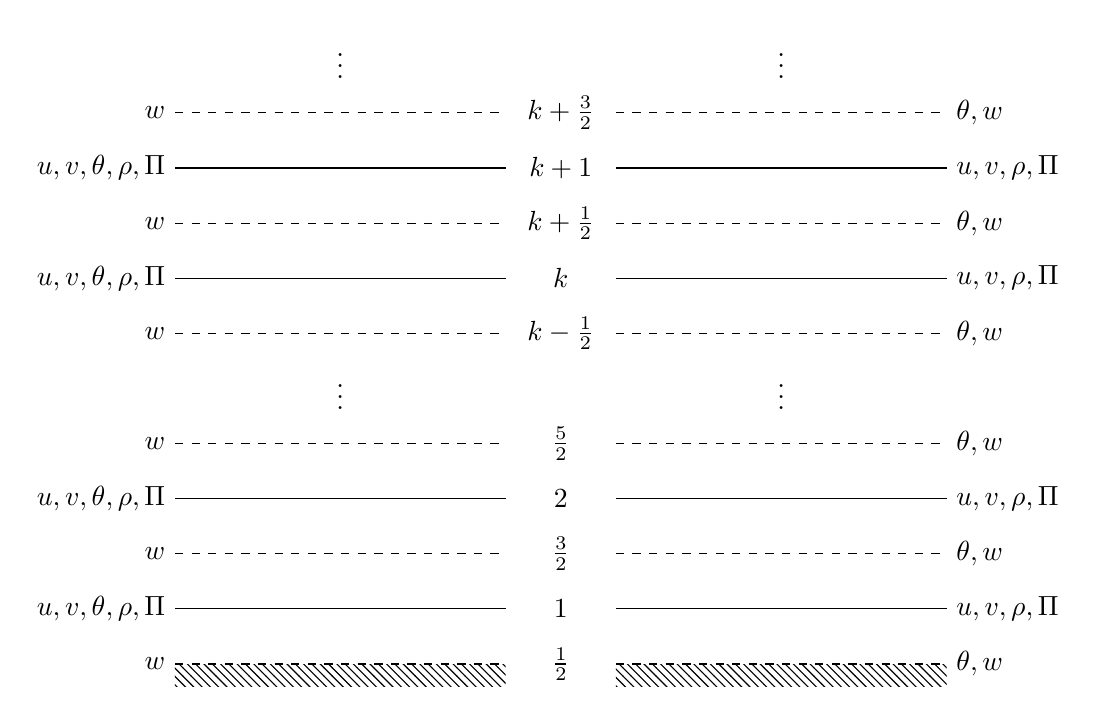
\begin{tikzpicture}[
  scale=0.7
]
\fill [pattern=north west lines] (0,0) rectangle (6,-0.4);
\fill [pattern=north west lines] (8,0) rectangle (14,-0.4);
\node at (7,0) {$\frac{1}{2}$};
\draw [dashed] (0,0) -- (6,0) node [at start, anchor=east] {$w$};
\draw [dashed] (8,0) -- (14,0) node [at end, anchor=west] {$\theta, w$};

\node at (7,1) {$1$};
\draw (0,1) -- (6,1) node [at start, anchor=east] {$u, v, \theta, \rho, \exner$};
\draw (8,1) -- (14,1) node [at end, anchor=west] {$u, v, \rho, \exner$};

\node at (7,2) {$\frac{3}{2}$};
\draw [dashed] (0,2) -- (6,2) node [at start, anchor=east] {$w$};
\draw [dashed] (8,2) -- (14,2) node [at end, anchor=west] {$\theta, w$};

\node at (7,3) {$2$};
\draw (0,3) -- (6,3) node [at start, anchor=east] {$u, v, \theta, \rho, \exner$};
\draw (8,3) -- (14,3) node [at end, anchor=west] {$u, v, \rho, \exner$};

\node at (7,4) {$\frac{5}{2}$};
\draw [dashed] (0,4) -- (6,4) node [at start, anchor=east] {$w$};
\draw [dashed] (8,4) -- (14,4) node [at end, anchor=west] {$\theta, w$};

\node at (3,5) {$\vdots$};
\node at (11,5) {$\vdots$};

\node at (7,6) {$k - \frac{1}{2}$};
\draw [dashed] (0,6) -- (6,6) node [at start, anchor=east] {$w$};
\draw [dashed] (8,6) -- (14,6) node [at end, anchor=west] {$\theta, w$};

\node at (7,7) {$k$};
\draw (0,7) -- (6,7) node [at start, anchor=east] {$u, v, \theta, \rho, \exner$};
\draw (8,7) -- (14,7) node [at end, anchor=west] {$u, v, \rho, \exner$};

\node at (7,8) {$k + \frac{1}{2}$};
\draw [dashed] (0,8) -- (6,8) node [at start, anchor=east] {$w$};
\draw [dashed] (8,8) -- (14,8) node [at end, anchor=west] {$\theta, w$};

\node at (7,9) {$k + 1$};
\draw (0,9) -- (6,9) node [at start, anchor=east] {$u, v, \theta, \rho, \exner$};
\draw (8,9) -- (14,9) node [at end, anchor=west] {$u, v, \rho, \exner$};

\node at (7,10) {$k + \frac{3}{2}$};
\draw [dashed] (0,10) -- (6,10) node [at start, anchor=east] {$w$};
\draw [dashed] (8,10) -- (14,10) node [at end, anchor=west] {$\theta, w$};

\node at (3,11) {$\vdots$};
\node at (11,11) {$\vdots$};
\end{tikzpicture}
\end{document}

	\caption{Lorenz (left) and Charney--Phillips (right) vertical staggering of variables.  Solid lines represent full levels, dashed lines represent half levels.  Adapted from \textcite{holdaway2013}.}
	\label{fig:theory:staggering}
\end{figure}

There are two commonly-used vertical staggerings, the Lorenz grid \autocite{lorenz1960} and the Charney--Phillips grid \autocite{charney-phillips1953}, which offer different sets of computational and physical properties.

In both grids, horizontal velocities $u$ and $v$, and density $\rho$, are stored at full levels, and the vertical velocity, $w$, is stored at half levels.  The two grids differ in their placement of potential temperature, $\theta$: on the Charney--Phillips grid it is stored at half levels, and at full levels on the Lorenz grid.  These arrangements of variables are summarised in figure~\ref{fig:theory:staggering}.  The placement of thermodynamic variables leads to different representations of hydrostatic balance in simulations of flows involving buoyancy.

The Charney--Philips grid was originally developed for a quasigeostrophic model using sigma coordinates.  \textcite{arakawa-moorthi1988} found that advection of quasi-geostrophic potential vorticity is conserved by this grid staggering, and it requires less interpolation of variables than the Lorenz grid \autocite{holdaway2013}. \TODO{anything else of significant interest to say about it?}

The Lorenz grid has a number of desirable properties: it conserves total energy, the mean potential temperature, and variance of potential temperature assuming no diabatic processes or friction \autocite{arakawa-konor1996}.  However, it is known that a computational mode exists on the Lorenz grid which can create a zig-zag in the vertical distribution of potential temperature \parencites{arakawa-moorthi1988}{arakawa-konor1996}{holdaway2013b}.  This can be explained by considering the vertical momentum equation \autocite{holdaway2013}
\begin{align}
	\frac{\partial w}{\partial t} + \vect{u} \cdot \del w = -g - c_p \theta \frac{\partial \exner}{\partial z}
\end{align}
where $\vect{u}$ is the velocity field, $g$ is the gravitational acceleration, $c_p$ is the heat capacity of dry air at constant pressure, $\theta = T \left( p_0 / p \right)^\kappa$ is the potential temperature, $T$ is the temperature, $\exner = \left( p / p_0 \right)^\kappa$ is the Exner function of pressure, $p$ is the pressure, $p_0$ is a reference pressure, $\kappa = R/c_p$, and $R$ is the specific gas constant of dry air.

\begin{figure}
	\centering
	\documentclass[tikz]{standalone}
\usepackage{bm}
\usetikzlibrary{patterns}
\newcommand{\vect}{\bm}
\newcommand{\del}{\nabla}

\newcommand{\trans}[1]{{#1^\star}}
\newcommand{\surface}{h}
\newcommand{\shellcmd}[1]{\texttt{#1}}
\newcommand{\diffusioncoeff}{\mathcal{D}}
\newcommand{\exner}{\Pi}
\newcommand{\courant}{\mathrm{Co}}

\begin{document}
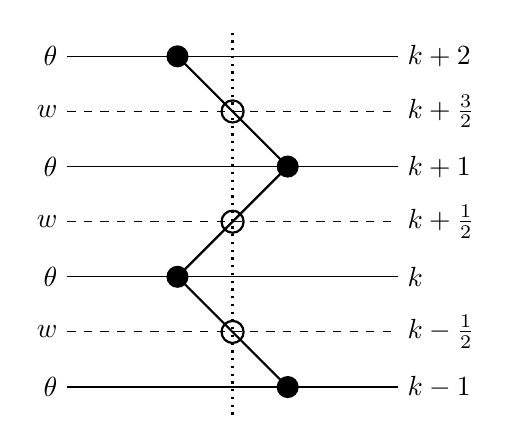
\begin{tikzpicture}[
  scale=0.7,
  cpnt/.style={fill=black}
]
\draw (0,0) -- (6,0) node [at start, anchor=east] {$\theta$} node [at end, anchor=west] {$k-1$};
\draw [dashed] (0,1) -- (6,1) node [at start, anchor=east] {$w$} node [at end, anchor=west] {$k-\frac{1}{2}$};
\draw (0,2) -- (6,2) node [at start, anchor=east] {$\theta$} node [at end, anchor=west] {$k$};
\draw [dashed] (0,3) -- (6,3) node [at start, anchor=east] {$w$} node [at end, anchor=west] {$k+\frac{1}{2}$};
\draw (0,4) -- (6,4) node [at start, anchor=east] {$\theta$} node [at end, anchor=west] {$k+1$};
\draw [dashed] (0,5) -- (6,5) node [at start, anchor=east] {$w$} node [at end, anchor=west] {$k+\frac{3}{2}$};
\draw (0,6) -- (6,6) node [at start, anchor=east] {$\theta$} node [at end, anchor=west] {$k+2$};

\path [cpnt] (4,0) circle [radius=0.2];
\path [cpnt] (2,2) circle [radius=0.2];
\path [cpnt] (4,4) circle [radius=0.2];
\path [cpnt] (2,6) circle [radius=0.2];
\draw [thick] (3,1) circle [radius=0.2];
\draw [thick] (3,3) circle [radius=0.2];
\draw [thick] (3,5) circle [radius=0.2];

\draw [thick] (4,0) -- (2,2) -- (4,4) -- (2,6);
\draw [thick, dotted] (3,-0.5) -- (3,6.5);
\end{tikzpicture}
\end{document}

	\caption{Interpolation of potential temperature on a Lorenz grid.  Solid circles denote values of $\theta$ stored at full levels and the solid line shows the potential temperature profile.  Open circles denote $\theta$ values interpolated onto half levels and the dotted line represents the interpolated profile.  Magnitude of $\theta$ increases to the right.}
	\label{fig:theory:theta-oscillation}
\end{figure}

In a discretisation of this equation, to calculate $w_{k+\frac{1}{2}}$, $\theta_{k+\frac{1}{2}}$ may be interpolated using an arithmetic mean of the adjacent values $\theta_k$ and $\theta_{k+1}$.  As shown in figure~\ref{fig:theory:theta-oscillation}, a grid-scale vertical wave in potential temperature would not be visible by the model \autocite{holdaway2013}.  Despite the oscillations, hydrostatic balance is satisfied and $w$ is everywhere zero.

The computational mode can affect the physical mode, causing spurious interactions with condensation processes \autocite{arakawa-konor1996} and the spurious generation of baroclinic instability and increased gravity wave activity \parencites{arakawa-moorthi1988}{cullen1997}.  The computational mode is not present on the Charney--Phillips grid.

